%%
%% This is file `sample-manuscript.tex',
%% generated with the docstrip utility.
%%
%% The original source files were:
%%
%% samples.dtx  (with options: `all,proceedings,bibtex,manuscript')
%% 
%% IMPORTANT NOTICE:
%% 
%% For the copyright see the source file.
%% 
%% Any modified versions of this file must be renamed
%% with new filenames distinct from sample-manuscript.tex.
%% 
%% For distribution of the original source see the terms
%% for copying and modification in the file samples.dtx.
%% 
%% This generated file may be distributed as long as the
%% original source files, as listed above, are part of the
%% same distribution. (The sources need not necessarily be
%% in the same archive or directory.)
%%
%%
%% Commands for TeXCount
%TC:macro \cite [option:text,text]
%TC:macro \citep [option:text,text]
%TC:macro \citet [option:text,text]
%TC:envir table 0 1
%TC:envir table* 0 1
%TC:envir tabular [ignore] word
%TC:envir displaymath 0 word
%TC:envir math 0 word
%TC:envir comment 0 0
%%
%% The first command in your LaTeX source must be the \documentclass
%% command.
%%
%% For submission and review of your manuscript please change the
%% command to \documentclass[manuscript, screen, review]{acmart}.
%%
%% When submitting camera ready or to TAPS, please change the command
%% to \documentclass[sigconf]{acmart} or whichever template is required
%% for your publication.
%%
%%
\documentclass[manuscript,screen,review]{acmart}
%%

\usepackage[hang,flushmargin]{footmisc}
\usepackage{amsmath}
\usepackage{amsthm}
\usepackage{verbatim}
\usepackage{enumitem}
\usepackage{multirow}
\usepackage{longtable}
\usepackage{booktabs} 
\usepackage{csquotes}
\usepackage{tikz}
\usetikzlibrary{arrows.meta,fit,positioning,shapes}
\usepackage{hyperref}
%
\newcommand\PO{\mathit{PO}}
\newcommand\Keys{\mathcal{K}}
\newcommand\nil{\varnothing}
\newcommand\defeq{\overset{\textrm{\tiny  def}}{=}}
\providecommand{\xor}{\veebar}
\newcommand{\idx}[1]{\texttt{[}\/#1\/\texttt{]}}
\DeclareMathOperator{\concat}{\operatorname{\oplus}}
\DeclareMathOperator{\Concat}{\operatornamewithlimits{\bigoplus}}
\DeclareMathOperator{\rangedel}{:}
\setlist[itemize]{label={---}}
% the following code puts a line break after a description label even if label is shorter than leftmargin
\renewcommand*{\descriptionlabel}[1]{\hspace\labelsep
\parbox{\linewidth}{#1}}
% \parbox{\linewidth}{\emph{#1}}}
\newlist{labelledlist}{description}{2}
\setlist[labelledlist]{style=nextline, leftmargin=2em, before=\renewcommand*{\descriptionlabel}[1]{\hspace\labelsep}}


%% \BibTeX command to typeset BibTeX logo in the docs
\AtBeginDocument{%
  \providecommand\BibTeX{{%
    Bib\TeX}}}

%% Rights management information.  This information is sent to you
%% when you complete the rights form.  These commands have SAMPLE
%% values in them; it is your responsibility as an author to replace
%% the commands and values with those provided to you when you
%% complete the rights form.
%\setcopyright{acmlicensed}
%\copyrightyear{2018}
%\acmYear{2018}
%\acmDOI{XXXXXXX.XXXXXXX}
%% These commands are for a PROCEEDINGS abstract or paper.
%\acmConference[Conference acronym 'XX]{Make sure to enter the correct
%  conference title from your rights confirmation email}{June 03--05,
%  2018}{Woodstock, NY}
%%
%%  Uncomment \acmBooktitle if the title of the proceedings is different
%%  from ``Proceedings of ...''!
%%
%%\acmBooktitle{Woodstock '18: ACM Symposium on Neural Gaze Detection,
%%  June 03--05, 2018, Woodstock, NY}
%\acmISBN{978-1-4503-XXXX-X/2018/06}


%%
%% Submission ID.
%% Use this when submitting an article to a sponsored event. You'll
%% receive a unique submission ID from the organizers
%% of the event, and this ID should be used as the parameter to this command.
%%\acmSubmissionID{123-A56-BU3}

%%
%% For managing citations, it is recommended to use bibliography
%% files in BibTeX format.
%%
%% You can then either use BibTeX with the ACM-Reference-Format style,
%% or BibLaTeX with the acmnumeric or acmauthoryear sytles, that include
%% support for advanced citation of software artefact from the
%% biblatex-software package, also separately available on CTAN.
%%
%% Look at the sample-*-biblatex.tex files for templates showcasing
%% the biblatex styles.
%%

%%
%% The majority of ACM publications use numbered citations and
%% references.  The command \citestyle{authoryear} switches to the
%% "author year" style.
%%
%% If you are preparing content for an event
%% sponsored by ACM SIGGRAPH, you must use the "author year" style of
%% citations and references.
%% Uncommenting
%% the next command will enable that style.
%%\citestyle{acmauthoryear}


%%
%% end of the preamble, start of the body of the document source.
\begin{document}

%%
%% The "title" command has an optional parameter,
%% allowing the author to define a "short title" to be used in page headers.
\title{Non-local redundancy: Erasure coding and dispersed replicas for robust retrieval in the Swarm peer-to-peer network}

%%
%% The "author" command and its associated commands are used to define
%% the authors and their affiliations.
%% Of note is the shared affiliation of the first two authors, and the
%% "authornote" and "authornotemark" commands
%% used to denote shared contribution to the research.
\author{Viktor Tr\'{o}n}
\authornote{Corresponding author}
\email{viktor@ethswarm.org}
\orcid{0009-0003-0222-6855}
% \affiliation{%
%   \city{Neuch\^{a}tel}
%   \institution{Swarm Research Division}
%   \country{Switzerland}
% }

\author{Viktor T\'{o}th}
\email{nugaon@ethswarm.org}
\affiliation{%
  \institution{Swarm Research Division}
  \city{Neuch\^{a}tel}
  \country{Switzerland}
}

\author{Gy\"{o}rgy Barab\'{a}s}
\email{gyorgy.barabas@liu.se}
\orcid{0000-0002-7355-3664}
\affiliation{%
  \institution{Division of Biology, Dept.~IFM, Link\"{o}ping University}
  \city{Link\"{o}ping}
  \country{Sweden}
}

\author{Callum Toner}
\email{callum@ethswarm.org}
% \affiliation{%
%   \institution{Swarm Research Division}
%   \city{Neuch\^{a}tel}
%   \country{Switzerland}
% }

\author{Daniel Nickless}
\email{dan@ethswarm.org}
% \email{sig32323232@gmail.com}
% \affiliation{%
%   \institution{Swarm Research Division}
%   \city{Neuch\^{a}tel}
%   \country{Switzerland}
% }

\author{D\'{a}niel A. Nagy}
\email{daniel@ethswarm.org}
% \affiliation{%
%   \institution{Swarm Research Division}
%   \city{Neuch\^{a}tel}
%   \country{Switzerland}
% }

\author{\'{A}ron Fischer}
\email{aron.fischer@gmail.com}
\affiliation{%
  \institution{Swarm Research Division}
  \city{Neuch\^{a}tel}
  \country{Switzerland}
}


%%
%% By default, the full list of authors will be used in the page
%% headers. Often, this list is too long, and will overlap
%% other information printed in the page headers. This command allows
%% the author to define a more concise list
%% of authors' names for this purpose.
\renewcommand{\shortauthors}{Tr\'{o}n et al.}

%%
%% The abstract is a short summary of the work to be presented in the
%% article.
\begin{abstract}
This paper presents an architecture for achieving resilient content retrieval in the Swarm decentralized storage network using erasure coding and non-local replication. The objective is to guarantee high data availability despite partial node failure or missing chunks. The proposed approach integrates Reed–Solomon coding into the Swarm hash tree, enabling the reconstruction of original data from a subset of stored chunks. Parametrized redundancy schemes are introduced to meet varying reliability requirements under various assumed rates of chunk retrieval failure. Dispersed replication of singleton chunks extends fault tolerance to edge cases. The paper also proposes retrieval strategies that exploit redundancy to optimize latency and cost. The result is a modular and practical design for robust file storage ideally suited for the adversarial and unreliable context of peer-to-peer decentralized networks.
\end{abstract}

%%
%% The code below is generated by the tool at http://dl.acm.org/ccs.cfm.
%% Please copy and paste the code instead of the example below.
%%
% \begin{CCSXML}
% <ccs2012>
%  <concept>
%   <concept_id>00000000.0000000.0000000</concept_id>
%   <concept_desc>Networks, Network algorithms</concept_desc>
%   <concept_significance>500</concept_significance>
%  </concept>
%  <concept>
%   <concept_id>00000000.00000000.00000000</concept_id>
%   <concept_desc>Networks, Network protocols</concept_desc>
%   <concept_significance>300</concept_significance>
%  </concept>
%  <concept>
%   <concept_id>00000000.00000000.00000000</concept_id>
%   <concept_desc>Information systems, Information storage systems</concept_desc>
%   <concept_significance>100</concept_significance>
%  </concept>
%  <concept>
%   <concept_id>00000000.00000000.00000000</concept_id>
%   <concept_desc>Do Not Use This Code, Generate the Correct Terms for Your Paper</concept_desc>
%   <concept_significance>100</concept_significance>
%  </concept>
% </ccs2012>
% \end{CCSXML}

\ccsdesc[500]{Networks~Network algorithms}
\ccsdesc[500]{Networks~Network protocols}
\ccsdesc[500]{Information systems~Information storage systems}

%%
%% Keywords. The author(s) should pick words that accurately describe
%% the work being presented. Separate the keywords with commas.
\keywords{Web3, Swarm, Decentralized storage, Erasure coding, Reed--Solomon encoding}

%\received{20 February 2007}
%\received[revised]{12 March 2009}
%\received[accepted]{5 June 2009}

%%
%% This command processes the author and affiliation and title
%% information and builds the first part of the formatted document.
\maketitle


This paper is structured as follows.
Section~\ref{sec:error-correcting-codes} introduces the role of erasure codes%
%
\footnote{\emph{Erasure codes} are error correcting techniques that have a focus on correcting data loss, rather than data corruption. They are a typical scheme of choice for distributed storage systems \citep{balaji2018erasure}.}
%
% in reliable data storage and the specific challenges faced in decentralised networks.
Section~\ref{sec:erasure} details the integration of Reed–Solomon encoding into the Swarm hash tree and explains how parity chunks are incorporated at each layer.
Section~\ref{sec:levels} provides a formal framework for selecting the number of parity chunks needed to meet predefined security thresholds, based on probabilistic failure models.
Section~\ref{sec:dispersed-replicas} addresses the special case of single-chunk redundancy by introducing dispersed replicas.
Section~\ref{sec:strategies} outlines retrieval strategies tailored for erasure-coded content, analyzing their respective trade-offs in terms of latency, cost, and robustness. Section~\ref{sec:conclusion} concludes.

\section{Introduction} \label{sec:error-correcting-codes}

Error correcting codes are widely utilized in the context of data  and storage to ensure data integrity in the face of a system fault. Error-correction schemes define how to rearrange or re-express data to add redundancy to its representation before upload or transmission (\emph{encoding}), so that corrupted data can be corrected or missing content reconstructed upon retrieval or reception (\emph{decoding}). The different schemes are evaluated by quantifying their strength (their \emph{tolerance} in terms of the sustainable rate of data corruption and loss) as a function of their cost (their \emph{overhead} in terms of storage and computation).

Specifically in the field of computer hardware architecture, synchronizing arrays of disks are crucial for providing resilient storage in data centers. %
%
In \emph{erasure coding}, %
%
%\footnote{\citep{buterin2014erasure}}
%
however, the problem can be framed as follows: How does one distribute data into \textit{shards} stored across the physical disks of an array or the physical nodes of a server cluster so that the data remains fully recoverable in the face of an arbitrary probability that any one or more physical carriers become faulty?

In the context of Swarm's distributed immutable \textit{chunk} store, DISC, the problem can be reformulated: How can data to be stored be encoded into chunks and distributed across \textit{neighborhoods}%
%
\footnote{Neighborhoods are groups of nodes which share responsibility for the same chunks.}
%
in the network so that the data remains fully recoverable in the face of an arbitrary probability that any one chunk is not retrievable?%
%
\footnote{We will assume that the retrieval of any one chunk fails with equal and independent probability.}

Reed-Solomon coding (RS)  \citep{reed1960polynomial,lubyetal1995CRS,plank2006optimizing,li2013erasure}
is the father of all  error correcting codes (ECC) and also the most widely used and implemented.%
%
\footnote{%
For a thorough comparison of an earlier generation of implementations of RS, see \citet{plank2009performance}.}
%
When applied to data of $m$ fixed-size blocks (a \emph{message} of length $m$), it produces an encoding of $m+k$ \emph{codewords} (blocks of the same size) in such a way that obtaining any $m$ out of the $m+k$ blocks is enough to reconstruct the original data. Conversely, $k$ puts an upper bound on the number of \emph{erasures} allowed (the number of unavailable blocks) for full recoverability, i.e., it expresses (the maximum) \emph{loss tolerance}.

$k$ is also the count of \emph{parities}, quantifying the data blocks added during the encoding on top of the original count of  blocks, in other words, it expresses the \emph{storage overhead}. While RS is optimal for storage (since loss tolerance cannot exceed the storage overhead), it has high bandwidth demands%
%
\footnote{Both the encoding and the decoding of RS codes takes $O(mk)$ time (with $m$ data chunks and $k$ parities). However, we found \emph{computational} overhead both insignificant for a network setting, as well as undifferentiating. The relevant metric is data size, as it determines both storage space and transmission bandwidth required.}
%
for local repair processes.%
%
\footnote{Entanglement codes \citep{estrada2018alpha, estrada2019building} require a minimal bandwidth overhead for a local repair, but at the cost of storage overhead that is in the multiples of $100\%$.}
%
The decoder needs to retrieve $m$ chunks to recover a particular unavailable chunk.
Hence, ideally, RS is used on files which are supposed to be downloaded in full,%
%
\footnote{Or in fragments large enough to include the data span over which the encoding is defined, such as videos.}
%
 but is much less appropriate for use cases needing only local repairs.%
%
\footnote{E.g., use cases requiring random access to small amounts of data (e.g., path lookups) benefit from simple replication, instead of RS, to optimise on bandwidth. Replication is, of course, suboptimal in terms of storage \citep{weatherspoon2002erasure}.}
%\enlargethispage{1.5cm}

When using RS, it is customary to use \emph{systematic} encoding, which means that the original data forms part of the encoding, with the parities added to it.%
%
%
\footnote{Our library of choice implementing exactly such a scheme is \url{https://github.com/klauspost/reedsolomon}.}


\section{Erasure coding in the Swarm hash tree}
\label{sec:erasure}

Swarm uses the \emph{Swarm hash tree} to represent files. This structure is a Merkle tree \citep{merkle1980protocols}, whose leaves constitute the consecutive segments of the input data stream. These segments are turned into chunks and are distributed among the Swarm nodes for storage. The consecutive chunk \emph{references} (either in the form of an address or an address and an encryption key) are recorded into chunks that represent a higher level. They are marked by special bits in the metadata that is part of every chunk, the 8-byte \emph{span}, which holds the byte-length for normal data chunks. 
These so-called \emph{packed address chunks} (PACs) constitute the intermediate chunks of the tree. PACs can point to data chunks or other PACs. The address of the top-most PAC is the root hash of the file, its unique, content-based address in the Swarm storage space. 
A branching factor $b$ is chosen so that the references to its children fill up a PAC fully.
With a reference (hash) size of 32 or 64 (hash plus encryption) and the fixed Swarm chunk size of 4096 bytes, the value of $b$ is thus 128 for unencrypted, and 64 for encrypted content
(Figure \ref{fig:Swarm-hash-split}).


\begin{figure}[!ht]
   \centering
   \input{Swarm-hash-split.tex}
   \caption[Swarm hash split]{The Swarm tree is the data structure encoding how a document is split into chunks.}
   \label{fig:Swarm-hash-split}
\end{figure}

Note that on the right edge of the hash tree, the last chunk of each level may be shorter than 4K: in fact, unless the file is exactly $4\cdot b^n$ kilobytes long, there is always at least one \emph{incomplete chunk}.  Importantly, it makes no sense to wrap a single chunk reference in a PAC. In these cases, it is attached to the first level. Such \emph{"dangling" chunks} will appear if and only if the file has a zero digit in its $b$-ary representation.

During file retrieval, a Swarm client starts from the root hash reference and retrieves the corresponding chunk. Interpreting the metadata, it decides that the chunk is a PAC if the span exceeds the maximum chunk size.
In case of a standard file download, all references packed within the PAC are followed and the referenced chunk data is retrieved.

PACs offer an organic and elegant way to implement consistent redundancy within the Swarm hash tree.
The input data for the erasure coding is the chunk data of the children, with the required equal-sized blocks corresponding to the chunk data of the consecutive references packed into the PAC. Instead of having each of the $b$ references packed represent children, only $m < b$ would, and the rest of the $k=b-m$ would encode RS parities (see Figure \ref{fig:Swarm-hash-erasure}).


The \emph{chunker} algorithm that implements PAC-scoped RS encoding would work as follows:
\begin{enumerate}[noitemsep]
\item Set the input to the actual data level and produce a sequence of chunks from the consecutive 4K segments of the data stream. Choose $m$ and $k$ such that $m+k=b$ is the branching factor (128 for unencrypted, and 64 for encrypted content).
\item Read the input one segment at a time. Count the segments by incrementing a counter $i$.
\item Repeat Step 2 until either $i = m$ or there is no more data left.
\item Use the RS scheme on the last $i\leq m$ chunks to produce $k$ parity chunks resulting in a total of $n = i+k \leq b$ chunks.
\item Concatenate the references of all these chunks to result in a packed address chunk (of size $h\cdot n$) on the level above. If this is the first chunk on that level, set the input to this level and spawn this same procedure from Step 2.
\item When the input is consumed, signal the end of input to the next-higher level and quit the routine. If there is no next-higher level, record the single chunk as the root chunk and use the reference to refer to the entire file.
\end{enumerate}

\begin{figure}[!ht]
   \centering
   \resizebox{1\textwidth}{!}{
        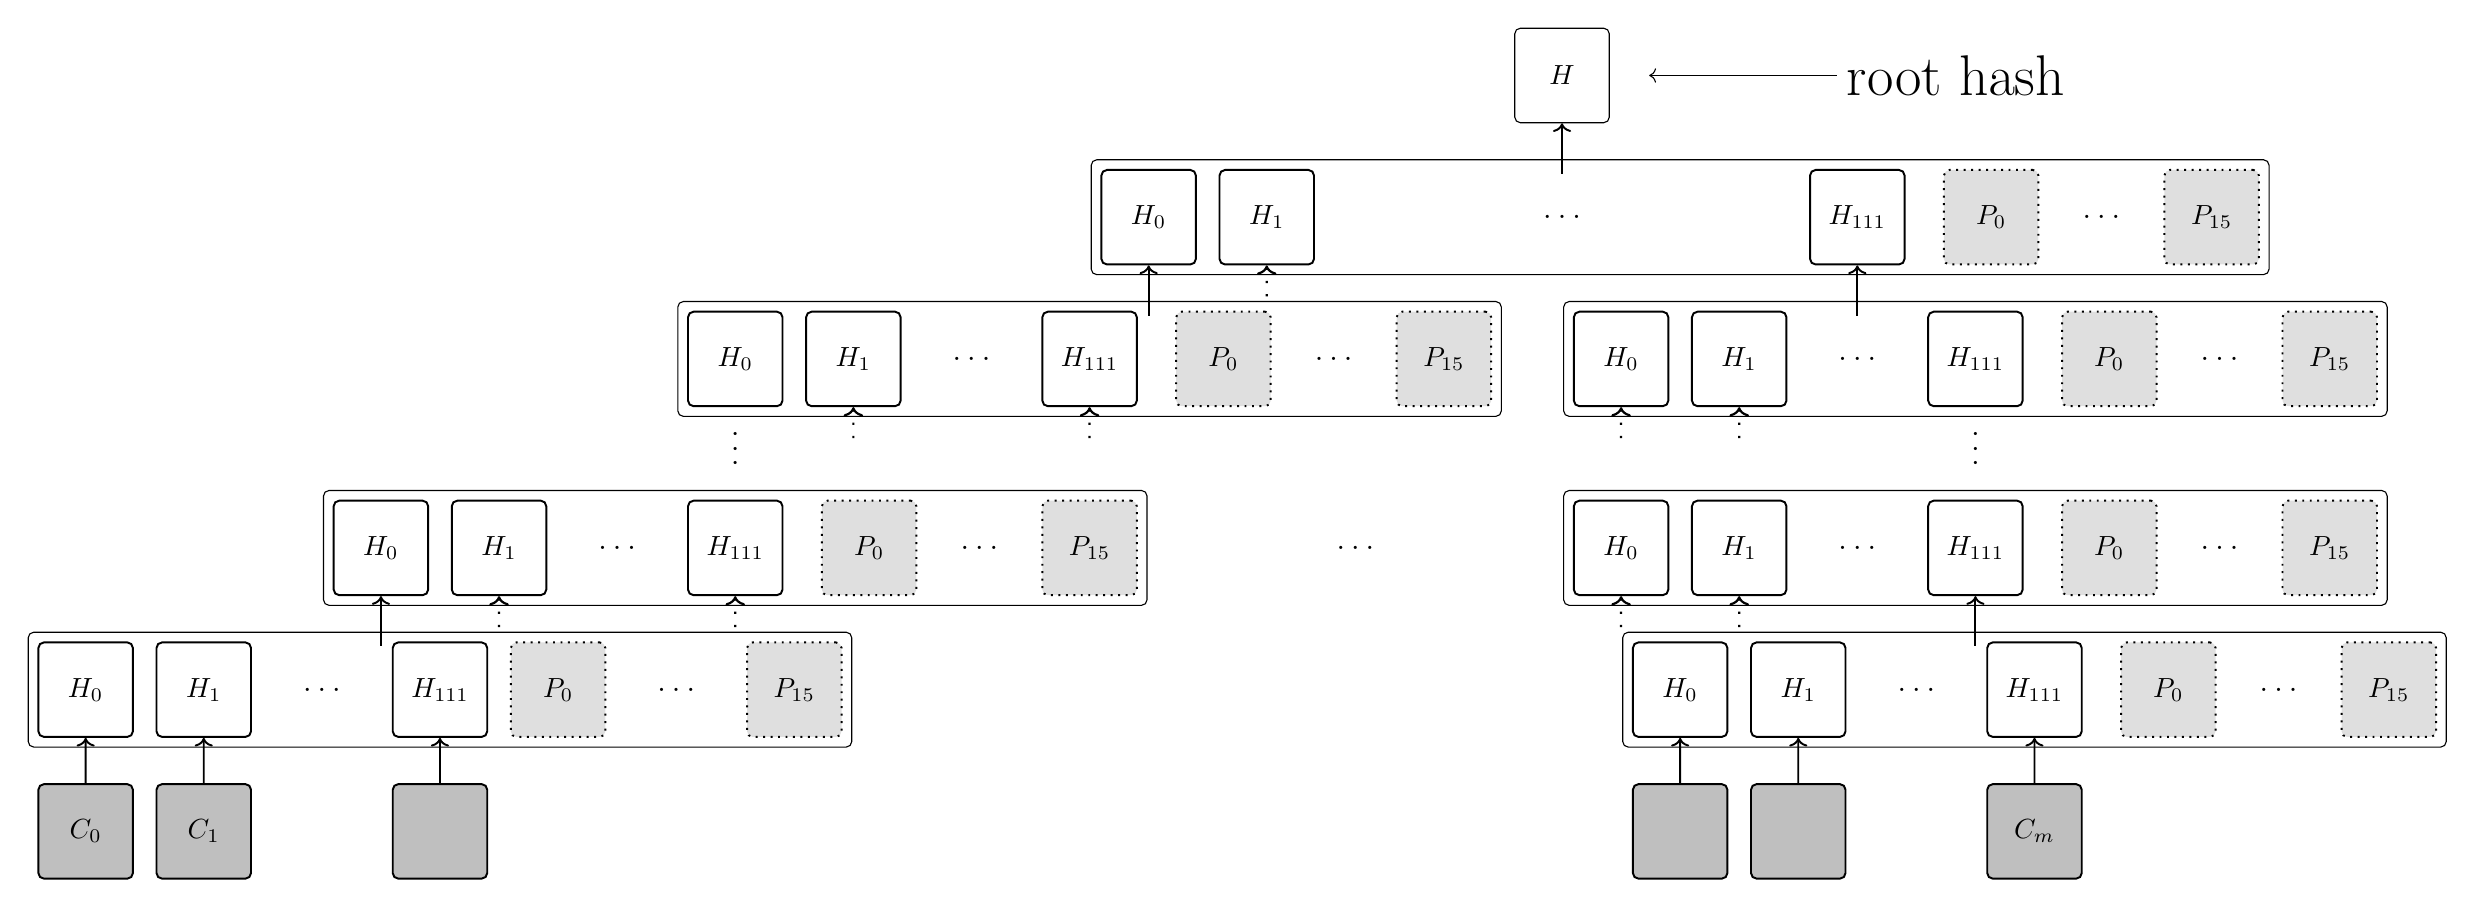
\begin{tikzpicture}[
level/.style={sibling distance=15mm, line width=0.7pt, level distance=18mm},
hash/.style={fill=white, rounded corners=2pt,draw,minimum size=1.2cm},
phash/.style={fill=lightgray!50, rounded corners=2pt,dotted,draw,minimum size=1.2cm},
chunk/.style={fill=lightgray, rounded corners=2pt,draw,minimum size=1.2cm},
midchunk/.style={draw=none,minimum size=0.2cm}
]

% root node
\node [hash] (root) {$H$}
  % vertical arrow
  child[grow=down,draw=none] { node {} edge from parent[<-,shorten >=12pt]}
  % annotation
  child[grow=right,draw=none,level distance=5cm] { node (swh) [font = {\huge} ] {root hash} edge from parent[draw=none] }
  % level n
  child {node [hash] (n-10) {$H_{0}$} edge from parent[draw=none]
    % arrow
    child[grow=down,draw=none] { node {} edge from parent[<-, shorten >=12pt]}
    % annotation
    % child[grow=left,draw=none,level distance=4cm] { node[align=center] at (-4,1) (bnl) {intermediate\\branching nodes\\chunks of 128 hashes}  edge from parent[draw=none] }
    % level n-1
    child {node [hash] (n-2l0) {$H_{0}$} edge from parent[draw=none]
      % level 2 compressed
      child[thick] {node [midchunk] (2l0) {} edge from parent[draw=none]
        % level 1
        child {node [hash] at (0,1.2) (1l0) {$H_{0}$} edge from parent[draw=none]
          % level 0
          child[grow=down,draw=none] { node {} edge from parent[<-, shorten >=12pt]}
          child {node [hash] (0l0) {$H_{0}$} edge from parent[<-, draw=none]
            child {node [chunk] {$C_{0}$}}
          }
          child {node [hash] (0l1) {$H_{1}$} edge from parent[<-, draw=none]
            child {node [chunk] (cl1) {$C_{1}$}}
          }
          child[missing]
          child {node [hash] (0ll) {$H_{111}$} edge from parent[<-, draw=none]
            child {node [chunk] (cll) {}}
          }
          child { node [phash] (p1-0ll) {$P_{0}$} edge from parent[draw=none]}
          child[missing]
          child { node [phash] (p15-0ll) {$P_{15}$} edge from parent[draw=none]}
        }
        % level 1 siblings
        child {node [hash] at (0,1.2) (1l1) {$H_{1}$} edge from parent[draw=none]
          child[thick,loosely dotted, shorten >=6mm, thick,<-] {node {}}
        }
        child[missing]
        child {node [hash] at (0,1.2) (1ll) {$H_{111}$} edge from parent[draw=none]
          child[thick,loosely dotted, shorten >=6mm, thick,<-] {node {}}
        }
        child { node [phash] at (0.2,1.2) (p1l) {$P_{0}$} edge from parent[draw=none]}
        child[missing]
        child { node [phash] at (0,1.2) (p1l0) {$P_{15}$} edge from parent[draw=none]}
      }
    }
    % level n-1 siblings lhs
    child {node [hash] (n-2l1) {$H_{1}$} edge from parent[draw=none]
      child[thick,loosely dotted, shorten >=6mm, thick,<-] {node {}}
    }
    child[missing]
    child {node [hash] (n-2ll) {$H_{111}$} edge from parent[draw=none]
      child[thick,loosely dotted, shorten >=6mm, thick,<-] {node {}}
    }
    child { node [phash] at (0.2,0) (p1-2ll) {$P_{0}$} edge from parent[draw=none]}
    child[missing]
    child { node [phash] (p15n-2ll) {$P_{15}$} edge from parent[draw=none]}
    child[missing]
    child[missing]
  }
  % level n siblings
  child {node [hash] (n-11) {$H_{1}$} edge from parent[draw=none]
    child[thick,loosely dotted, shorten >=6mm, thick,<-] {node {}}
  }
  child[missing]
  child[missing]
  child[missing]
  child[missing]
  child { node [hash] (n-1l) {$H_{111}$} edge from parent[draw=none]
    % level n-2 siblings rhs vertical arrow
    child[grow=down,draw=none] { node {} edge from parent[<-, shorten >=12pt]}
    % child[grow=right,level distance=9cm] { node[align=center] (bnr)   {intermediate\\branching nodes\\chunks of 128 hashes}edge from parent[draw=none]}
    child[missing]
    child {node [hash] (n-2r0) {$H_{0}$} edge from parent[draw=none]
      child[thick,loosely dotted, shorten >=6mm, thick,<-] {node {}}
    }
    child {node [hash] (n-2r1) {$H_{1}$} edge from parent[draw=none]
      child[thick,loosely dotted, shorten >=6mm, thick,<-] {node {}}
    }
    child[missing]
    child {node [hash] (n-2rl) {$H_{111}$} edge from parent[draw=none]
      % level 2 siblings compressed
      child[grow=down] {node [midchunk] (2rl) {} edge from parent[draw=none]
        % level 1 siblings moved up
        child {node [hash] at (0,1.2) (1r0) {$H_{0}$} edge from parent[draw=none]
          child[thick,loosely dotted, shorten >=6mm, thick,<-] {node {}}
        }
        child {node [hash] at (0,1.2) (1r1) {$H_{1}$} edge from parent[draw=none]
          child[thick,loosely dotted, shorten >=6mm, thick,<-] {node {}}
        }
        child[missing]
        child {node [hash] at (0,1.2) (1rl) {$H_{111}$} edge from parent[draw=none]
          % level 0 siblings rhs
          child[grow=down,draw=none] { node {} edge from parent[<-, shorten >=12pt]}
          child {node [hash] (0r0) {$H_{0}$} edge from parent[<-, draw=none]
            child {node [chunk] (cr0) {}}
          }
          child {node [hash] (0r1) {$H_{1}$} edge from parent[<-, draw=none]
            child {node [chunk] (cr1) {}}
          }
          child[missing]
          child {node [hash] (0rl) {$H_{111}$} edge from parent[<-, draw=none]
            child {node [chunk] (crl) {$C_{m}$}
            %   child [grow=right] { edge from parent[draw=none]
            %     child [grow=right] {node[align=center] {leaf chunks\\data level} edge  from parent[draw=none]
            %       child [grow=up] {node {level $0$} edge from parent[draw=none]
            %         child [grow=up] {node {level $1$} edge from parent[draw=none]
            %             child [grow=up] {node at (0,0.8) {level $n-1$} edge from  parent[draw=none]
            %               child [grow=up] {node {root = level $n$} edge from  parent[draw=none]}
            %             }
            %         }
            %       }
            %     }
            %   }
            }
          }
          child { node [phash] at (0.2,0) (p100) {$P_{0}$} edge from parent[draw=none]}
          child[missing]
          child { node [phash] (p150) {$P_{15}$} edge from parent[draw=none]}
        }
        child { node [phash] at (0.2,1.2) (p11) {$P_{0}$} edge from parent[draw=none]}
        child[missing]
        child { node [phash] at (0,1.2) (p151) {$P_{15}$} edge from parent[draw=none]}
      }
    }
    child { node [phash] at (0.2,0) (p1n-2) {$P_{0}$} edge from parent[draw=none]}
    child[missing]
    child { node [phash] (p15n-2) {$P_{15}$} edge from parent[draw=none]}
  }
  child { node [phash] at (0.2,0) (p1n) {$P_{0}$} edge from parent[draw=none]}
  child[missing]
  child { node [phash] (p15n-11) {$P_{15}$} edge from parent[draw=none]};

% elipsis
\path (p1n) -- (p15n-11) node [midway,font=\large] {$\ldots$};
\path (p1n-2) -- (p15n-2) node [midway,font=\large] {$\ldots$};
\path (p11) -- (p151) node [midway,font=\large] {$\ldots$};
\path (p100) -- (p150) node [midway,font=\large] {$\ldots$};
\path (p1l) -- (p1l0) node [midway,font=\large] {$\ldots$};
\path (p1-0ll) -- (p15-0ll) node [midway,font=\large] {$\ldots$};
\path (p1-2ll) -- (p15n-2ll) node [midway,font=\large] {$\ldots$};


\path (n-11) -- (n-1l) node [midway,font=\large] {$\ldots$};
\path (n-2l0) -- (2l0) node [midway,font=\large,sloped] {$\ldots$};
\path (n-2rl) -- (2rl) node [midway,font=\large,sloped] {$\ldots$};
\path (1l1) -- (1ll) node [midway,font=\large] {$\ldots$};
\path (1r1) -- (1rl) node [midway,font=\large] {$\ldots$};
\path (p1l0) -- (1r0) node [midway,font=\large] {$\ldots$};
\path (n-2l1) -- (n-2ll) node [midway,font=\large] {$\ldots$};
\path (n-2r1) -- (n-2rl) node [midway,font=\large] {$\ldots$};
% \path (n-2ll) -- (n-2r0) node [midway,font=\large,sloped] {$\ldots$};
\path (0l1) -- (0ll) node [midway,font=\large] {$\ldots$};
\path (0r1) -- (0rl) node [midway,font=\large] {$\ldots$};
% \path (0ll) -- (0r0) node [midway,font=\large] {$\ldots$};
% \path (cl1) -- (cll) node [midway,font=\large] {$\ldots$};
% \path (cr1) -- (crl) node [midway,font=\large] {$\ldots$};
% \path (cll) -- (cr0) node [midway,font=\large] {$\ldots$};
% \path (p1) -- (p15) node [midway,font=\large] {$\ldots$};


% arrows from annotations
\begin{scope}[shorten >=.5cm,thin]
\draw [->] (swh) -> (root);
% \draw [->] (bnl) -> (n-10);
% \draw [->] (bnl) -> (n-2l0);
% \draw [->] (bnl) -> (1l0);
% \draw [->] (bnl) -> (0l0);
% \draw [->] (bnr) -> (n-1l);
% \draw [->] (bnr) -> (n-2rl);
% \draw [->] (bnr) -> (1rl);
% \draw [->] (bnr) -> (0rl);
\end{scope}

% boxes to group nodes
% \node[rounded corners=2pt, draw=white, minimum height=1.1cm, fit=(root)] {};
\node[rounded corners=2pt, draw=black, minimum height=1.1cm, fit=(n-10) (p15n-11)] {};

\node[rounded corners=2pt, draw=black, minimum height=1.1cm, fit=(0l0) (p15-0ll)] {};
\node[rounded corners=2pt, draw=black, minimum height=1.1cm, fit=(n-2l0) (p15n-2ll)] {};
\node[rounded corners=2pt, draw=black, minimum height=1.1cm, fit=(n-2r0) (p15n-2)] {};
\node[rounded corners=2pt, draw=black, minimum height=1.1cm, fit=(1l0) (p1l0)] {};
\node[rounded corners=2pt, draw=black, minimum height=1.1cm, fit=(1r0) (p151)] {};

\node[rounded corners=2pt, draw=black, minimum height=1.1cm, fit=(0r0) (p150)] {};

\end{tikzpicture}

   }
   \caption[Swarm hash erasure]{An unencrypted Swarm tree with $k=16$ extra parity chunks using $m=112$ out of $n=128$ RS encoding. Chunks $P_{0}$ through $P_{15}$ are parity data for chunks $H_0 $ through $H_{111}$ on every level of intermediate chunks. This pattern repeats itself all the way down the tree. Thus, hashes $H_{m+1}$ through $H_{127}$ point to parity data for chunks pointed to by $H_0$ through $H_{m}$. Since parity chunks $P_i$ do not have children, the tree structure does not have uniform depth.}
   \label{fig:Swarm-hash-erasure}
\end{figure}

\section{Levels of security and the number of parities}\label{sec:levels}

Non-local redundancy is presented here as a scheme of encoding that allows strategies of retrieval in order to guarantee data availability.
With packed address chunks as the scope of erasure codes, it is crucial that we use the right number of shards and parities among the children of an intermediate node in the Swarm hash tree representing a file to achieve the desired robustness.
Given assumptions about chunk retrieval error rates and the number of parities used, one can calculate, the degree of certainty that the data can be recovered without error. One can even apply the same logic backwards: given some level of certainty with which we want recovery to be error-free, we can compute how many parities should be used.
In what follows, we give a formal exposition of how to find these parity counts.


Let there be $m$ original chunks and $k$ parity chunks, such that any $m$ chunks out of the total $n = m + k$ ones are fully recoverable after the loss of any $k$ of them. In the process of retrieving the $n$ chunks, what is the likelihood of overall data corruption, given a per-chunk probability of error $\epsilon$?

By ``overall data corruption'', we mean that more than $k$ chunks are damaged or unavailable in the data retrieval process. We assume that each chunk's probability of error is independent of other chunks. In that case, the problem boils down to the independent drawing of $n$ chunks, each of which undergo a \emph{Bernoulli trial} of being faulty with probability $\epsilon$. The probability of a number of chunks out of $n$ independent Bernoulli trials being faulty is given by the \emph{binomial distribution}:
\begin{equation}
  B(i, n, \epsilon) = \binom{n}{i} \epsilon^i (1-\epsilon)^{n-i} .
  \label{eq-PMF-binomial}
\end{equation}
This expression is the probability mass function for the binomial distribution, yielding the probability that out of $n$ chunks, exactly $i$ will be faulty---assuming that the per-chunk probability of error is $\epsilon$.

Since there are $k$ parities out of the $n$ chunks, the system can tolerate up to $k$ chunk errors. The probability that no more than $k$ errors accumulate can be expressed by summing Equation~\ref{eq-PMF-binomial} over $i$ up to $k$:
\begin{equation}
  P(k, n, \epsilon) = \sum_{i=0}^k \binom{n}{i} \epsilon^i (1-\epsilon)^{n-i} ,
  \label{eq-CDF-binomial}
\end{equation}
which is the cumulative distribution function of the binomial distribution.

One typical question is the following: given the number of chunks $n$ and a value $\alpha$ such that we want the overall probability of data corruption to be below this value, how many out of the $n$ chunks should be parities? Since $P(k, n, \epsilon)$ is the probability that \emph{no more than} $k$ errors accumulate, $1 - P(k, n, \epsilon)$ is the probability of more than $k$ errors; i.e., that \emph{at least} $k + 1$ errors accumulated and therefore a file cannot be retrieved in its entirety. We want to keep this probability below $\alpha$, so we can write
\begin{equation}
  \alpha \ge 1 - P(k, n, \epsilon) .
  \label{eq-CDF-cond}
\end{equation}
Rearranging, we have
\begin{equation}
  1 - \alpha \le P(k, n, \epsilon) .
  \label{eq-CDF-cond2}
\end{equation}
That is, we are looking for values of $k$ which will satisfy this inequality (cf. figure \ref{fig:alpha}). This can be obtained by inverting the cumulative distribution function in $k$, resulting in the quantile function $Q(1 - \alpha, n, \epsilon)$. While this inverse has no convenient closed-form expression, it can be efficiently evaluated numerically for any set of input parameters. As with any cumulative distribution function, $P(k, n, \epsilon)$ is monotonically increasing in $k$. Applying the inverse on both sides of Equation~\ref{eq-CDF-cond2} therefore does not flip the direction of the inequality, and gives $k \ge Q(1 - \alpha, n, \epsilon)$. Or if we look for the smallest $k$ satisfying this condition:
\begin{equation}
  k_{min} = Q(1 - \alpha, n, \epsilon) .
  \label{eq-quantile-sol-n}
\end{equation}
This is the formula yielding the minimum number of required parities to keep the overall probability of data corruption below $\alpha$.

\begin{figure}[!ht]
  \centering
  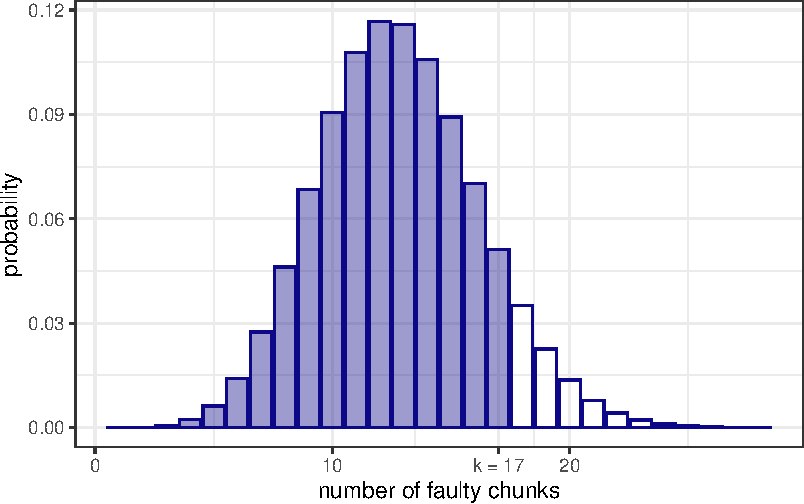
\includegraphics[width=.7\textwidth]{fig-alpha-1.pdf}
  \caption{The point at $k=17$ along the binomial distribution, where the probability of exceeding this many errors becomes less than $\alpha = 10\%$. This cumulated probability is the area under the curve right of $x=17$. For this example, the total number of chunks is $n = 128$, and the per-chunk error rate assumed is $\epsilon = 0.1$.}
  \label{fig:alpha}
\end{figure}

Figure \ref{fig:perr-lin} presents the number of parities needed as a function of error rate for various levels of security.
\begin{figure}[!ht]
  \centering
  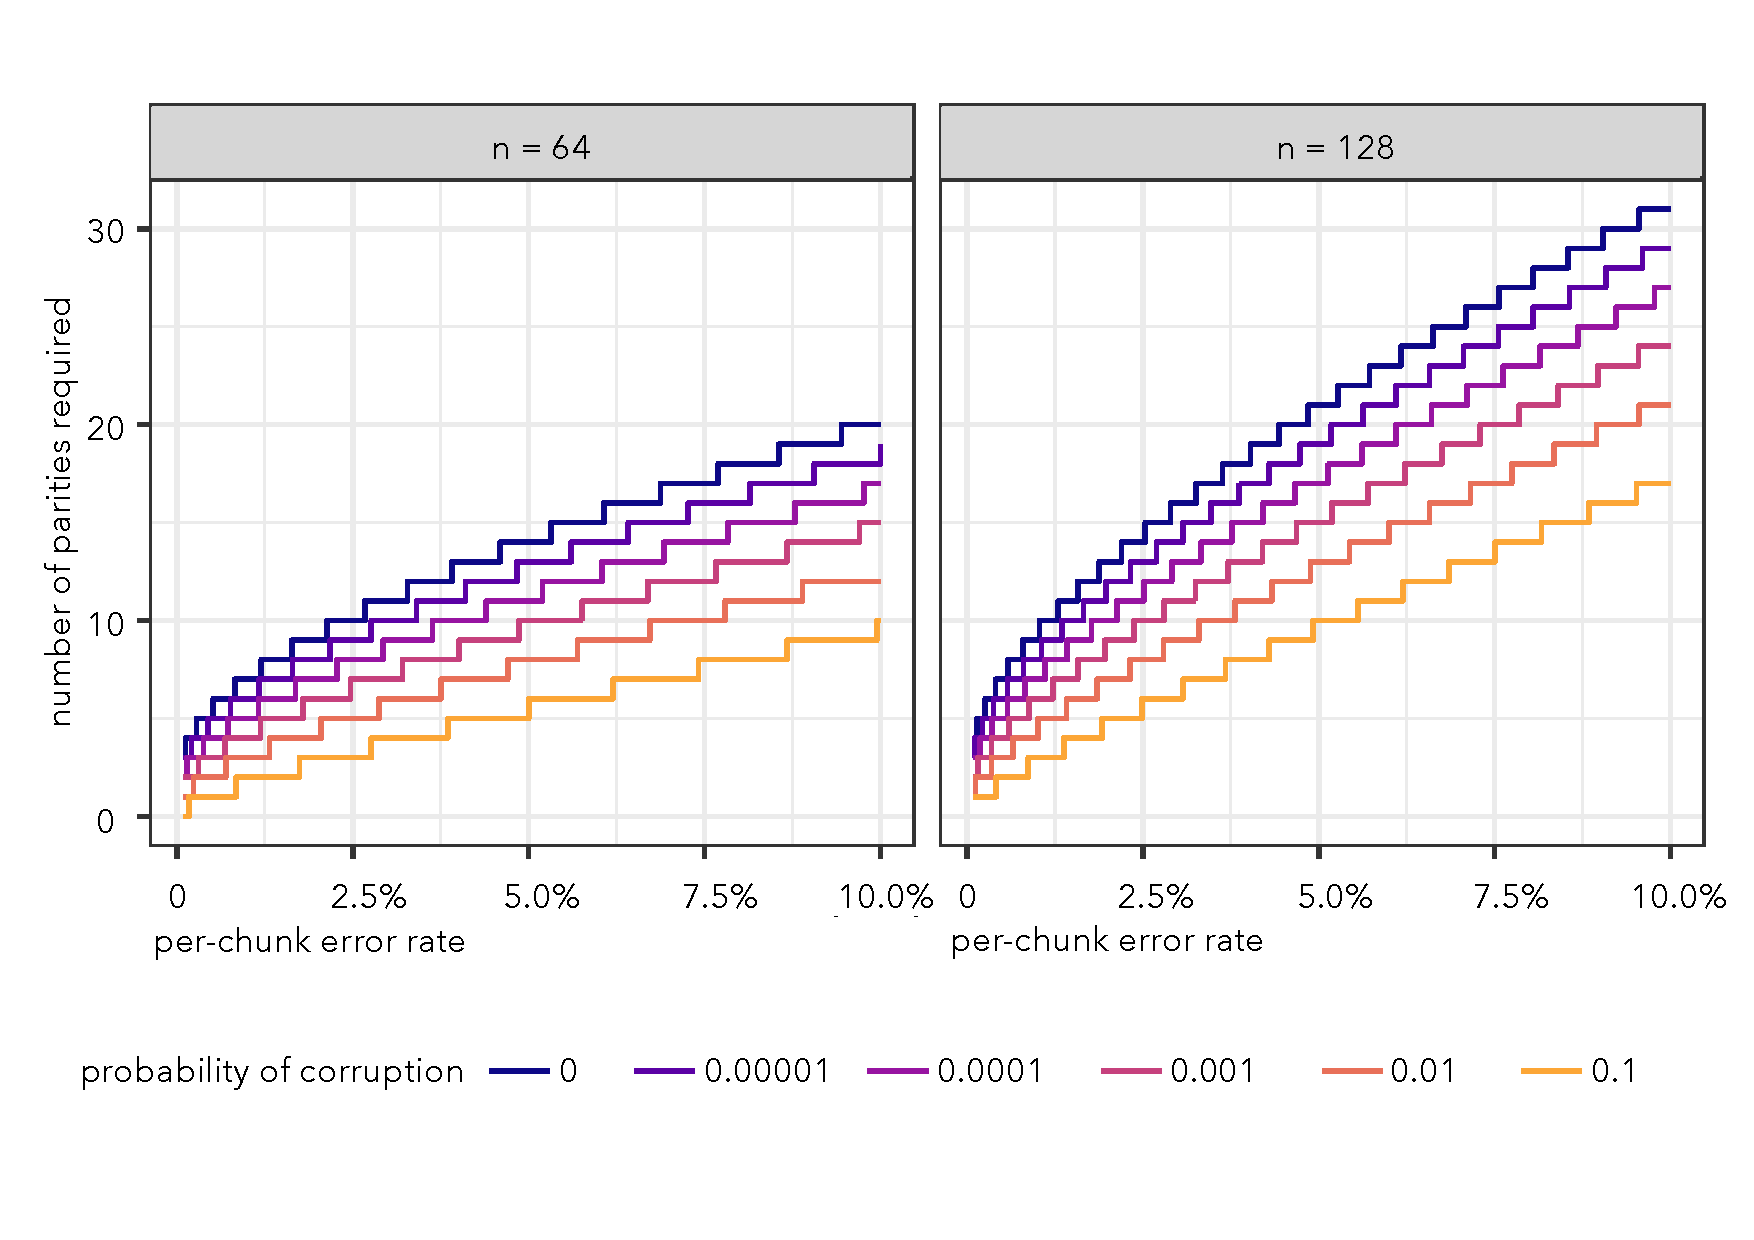
\includegraphics[width=.85\textwidth]{fig-perr-lin-1.1.4-flat-crop.pdf}
  \caption{The number of parities needed (ordinate) as a function of the per-chunk error rate $\epsilon$ (abscissa), for keeping the probability of overall data corruption below given limits (colours) and for $n = 64$ chunks (left panel) and $n = 128$ chunks (right panel).}
  \label{fig:perr-lin}
\end{figure}
Figure \ref{fig:integrity}  
presents the number of parities needed to keep the probability of overall data corruption at a given level for various values of the per-chunk error rate.
\begin{figure}[!ht]
  \centering
  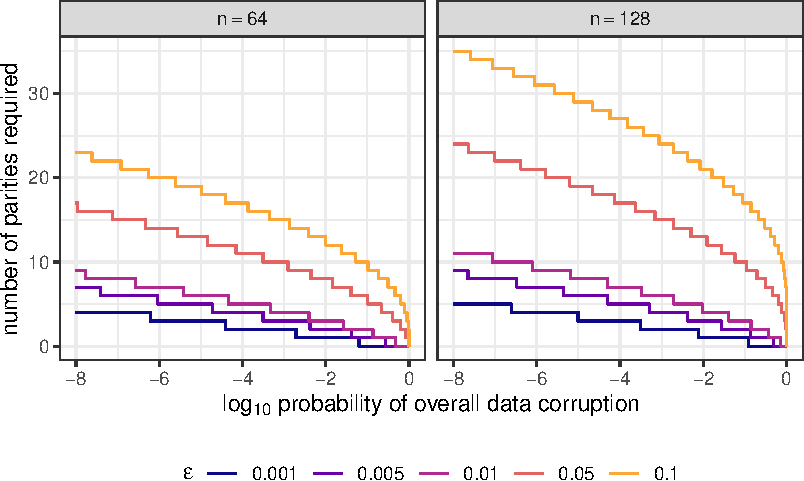
\includegraphics[width=.7\textwidth]{fig-integrity-1.pdf}
  \caption{The number of parities required (ordinate) to keep the probability of overall data corruption at a given level (abscissa), for various values of the per-chunk error rate $\epsilon$ (colours) and for $n = 64$ chunks (left panel) and $n = 128$ chunks (right panel).}
  \label{fig:integrity}
\end{figure}

The same type of problem can also be phrased slightly differently: given a number of chunks $n$, how many parities $k$ should be added to them to keep the overall data corruption probability below some level $\alpha$? In this case, the total number of chunks is $n + k$ (instead of having $n$ chunks, out of which $k$ are parities), and so Equation~\ref{eq-quantile-sol-n} is modified to be
\begin{equation}
  k = Q(1 - \alpha, n + k, \epsilon) .
  \label{eq-quantile-sol}
\end{equation}
While this equation has no closed-form solution for $k$, one can easily find the $k$ satisfying it as long as $k$ is bounded in a relatively small range. In our case, the maximum number of chunks, $n + k$, is 128, and so $k$ is at most $128-n$. This makes it simple to find the value of $k$ compatible with Equation~\ref{eq-quantile-sol}. The number of parities in Tables~\ref{tbl:levels}-\ref{tbl:paranoid} were obtained using this method.

In principle, the exact parity counts can be made user-configurable. However, to make non-local redundancy a transparent and easy-to-use feature, we opted for a simplified yet intuitive interface.
First of all, we set our maximum tolerated error rate of integrity at $10^{-6}$, in other words our security constant expressing our certainty at 6 nines, 99.9999\%.
Second, we propose to use a handful of named security levels of (non-local) redundancy which correspond to assumptions about the maximum error rates of individual chunk retrievals expressed as discrete percentages. 
Table~\ref{tbl:levels} lists the security levels with the  corresponding assumption about the maximum error rate of chunk retrieval. 
\begin{table}[!ht]
\centering
\caption{Security levels for non-local redundancy UI and corresponding assumptions about uniform and independent error rates of individual chunk retrieval. In subsequent columns we specify the composition of full chunks for the security levels for unencrypted (columns 4 and 5) and encrypted (columns 6 and 7) content.}
\begin{tabular}{|c|c|r||r|r|r|r|}
\hline
\multicolumn{2}{|c|}{security}
&\multirow{2}{3.3cm}{\centering presumed error rate\\of chunk retrieval}
&\multicolumn{2}{|c|}{unencrypted}
&\multicolumn{2}{|c|}{encrypted}\\\cline{1-2}\cline{4-7}
level&name&
& chunks & parities 
& chunks & parities 
\\\hline
0     & \textsc{none} &       0\% &   128 &   0 &  64 &   0 \\
1     & \textsc{medium} &     1\% &   119 &   9 &  59 &   9 \\
2     & \textsc{strong} &     5\% &   107 &  21 &  53 &  21 \\
3     & \textsc{insane} &    10\% &    97 &  31 &  48 &  31 \\
4     & \textsc{paranoid} &  50\% &    38 &  90 &  19 &  90 \\
\hline
\end{tabular}
\label{tbl:levels}
\end{table}

% \section{Incomplete chunks and parity counts}
If the number of file chunks is not a multiple of $m$, it is not possible to proceed with the last batch in the same way as the others. We propose that we encode the remaining chunks with an erasure code that guarantees at least the same level of security as the others.%
%
\footnote{Note that this is not as simple as choosing the same redundancy. For example, a $50\text{-out-of-}100$ encoding is much more secure against loss than a $1\text{-out-of-}2$ encoding, even though the redundancy is $100\%$ in both cases.}
%
Overcompensating, we still require the same number of parity chunks even when there are fewer than $m$ data chunks. However, we can also just calculate the necessary parities for all possible incomplete chunks and security levels. Figure~\ref{fig:maintain} plots the number of parities against the number of chunks required:


\begin{figure}[!ht]
  \centering
  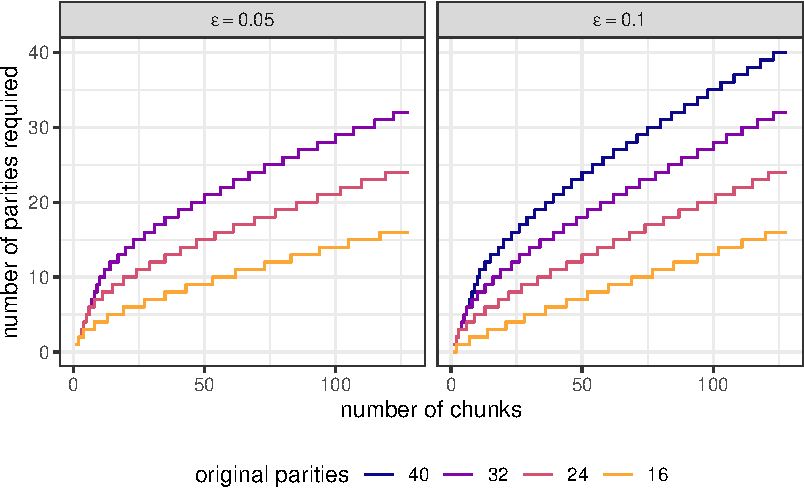
\includegraphics[width=.8\textwidth]{fig-maintain-1.pdf}
  \caption{Number of chunks (abscissa) and the corresponding required number of parities (ordinate) such that will maintain the same overall probability of no data corruption as would be the case with 128 chunks, an original number of parities indicated by the colours, and a likelihood $\epsilon$ of an erroneous retrieval of a single chunk indicated in the panel headers.}
  \label{fig:maintain}
\end{figure}

Tables~\ref{tbl:parities} and \ref{tbl:paranoid} show 
the number of chunks that are maintainable for a given number of parities $k$ across various security levels.
Since encrypted chunks are referenced with the hash address followed by the decryption key, an encrypted reference takes up 2 hash-sized segments. Parity chunks added to an encrypted PAC, however, are calculated based on the encrypted shards and are themselves not encrypted, hence their references only use a single hash. 
Thus, the number of effective hash-sized segments 
used is obtained as twice the number of chunks plus the number of parities. Since this can be an odd number and less than 128, in some security levels even the full chunks are not completely full.


\begin{table}[!ht]
\centering
\caption{The number of parities (first column in each table) to be appended to a given number of chunks (second and third column of each table, given as a range) so that the probability of an unsuccessful data retrieval remains below $\alpha = 10^{-6}$. The second column is for unencrypted  chunks, while the third one is for encrypted chunks. The tables are for security levels 1-3, to be continued for security level 4 in Table~\ref{tbl:paranoid}.}
\begin{minipage}{.49\linewidth}
\begin{tabular}{|r|r|r|}
\multicolumn{3}{c}{\textsc{medium}}\\\hline
\multirow{2}{1.5cm}{\centering 
 parities } 
&\multicolumn{2}{|c|}{ chunks }\\\cline{2-3}
&\multicolumn{1}{|c|}{unencrypted}
&\multicolumn{1}{|c|}{encrypted} \\\hline\hline
2 & 1 & - \\
3 & 2-5     & 1-2\\
4 & 6-14    & 3-7\\ 
5 & 15-28   & 7-14\\ 
6 & 29-46   & 14-23\\  
7 & 47-68   & 23-34\\  
8 & 69-94   & 34-47\\  
9 & 95-119  & 47-59\\   
\hline
%
\multicolumn{3}{c}{\textsc{}}\\
\multicolumn{3}{c}{\textsc{strong}}
\\\hline
4 & 1   &  -\\
5 & 2-3   & 1\\
6 & 4-6   & 2-3\\
7 & 7-10  & 3-5\\
8 & 11-15 & 5-7\\
9 & 16-20 & 8-10\\
10 & 21-26 & 10-13\\
11 & 27-32 & 13-16\\
12 & 33-39 & 16-19\\
13 & 40-46 & 20-23\\
14 & 47-53 & 23-26\\
15 & 54-61 & 27-30\\
16 & 62-69 & 31-34\\
17 & 70-77 & 35-38\\
18 & 78-86 & 39-43\\
19 & 87-95 & 43-47\\
20 &96-104 & 48-52\\
21&105-107 & 52-53\\
\hline
\end{tabular}
\end{minipage}
\begin{minipage}{.49\linewidth}
\centering
\begin{tabular}{|r|r|r|}
\multicolumn{3}{c}{\textsc{}}\\
\multicolumn{3}{c}{\textsc{insane}}\\\hline
\multirow{2}{1.5cm}{\centering 
 parities } 
&\multicolumn{2}{|c|}{ chunks }\\\cline{2-3}
&\multicolumn{1}{|c|}{unencrypted} 
&\multicolumn{1}{|c|}{encrypted} \\\hline\hline
5 & 1     &-   \\
6 & 2     & 1\\
7 & 3     & 1\\ 
8 & 4-5   & 2\\ 
9 & 6-8   & 3-4\\
10 & 9-10  & 4-5\\
11 & 11-13 & 5-6\\
12 & 14-16 & 7-8\\
13 & 17-19 & 8-9\\
14 & 20-22 & 10-11\\
15 & 23-26 & 11-13\\
16 & 27-29 & 13-14\\
17 & 30-33 & 15-16\\
18 & 34-37 & 17-18\\
19 & 38-41 & 19-20\\
20 & 42-45 & 21-22\\
21 & 46-50 & 23-25\\
22 & 51-54 & 25-27\\
23 & 55-59 & 27-29\\
24 & 60-63 & 30-31\\
25 & 64-68 & 32-34\\
26 & 69-73 & 34-36\\
27 & 74-77 & 37-38\\
28 & 78-82 & 39-41\\
29 & 83-87 & 41-43\\
30 & 88-92 & 44-46\\
31 & 93-97 & 46-48\\
\hline
\multicolumn{3}{c}{}\\
\multicolumn{3}{c}{}
\end{tabular}
\end{minipage}
\label{tbl:parities}
\end{table}


\begin{table}[!ht]
\caption{As Table~\ref{tbl:parities}, but for the \textsc{paranoid} security level.}
\begin{minipage}{.49\linewidth}
\centering
\begin{tabular}{|r|r|r|}
\multicolumn{3}{c}{\textsc{}}\\
\multicolumn{3}{c}{\textsc{paranoid}}\\\hline
\multirow{2}{1.5cm}{\centering 
 parities } 
&\multicolumn{2}{|c|}{ chunks }\\\cline{2-3}
&\multicolumn{1}{|c|}{unencrypted} 
&\multicolumn{1}{|c|}{encrypted} \\\hline\hline
19 & 1 & -\\
23 & 2  & 1\\
26 & 3  & 1\\
29 & 4  & 2\\
31 & 5  & 2\\
34 & 6  & 3\\
36 & 7  & 3\\
38 & 8  & 4\\
40 & 9  & 4\\
43 & 10 & 5\\
45 & 11 & 5\\
47 & 12 & 6\\
48 & 13 & 6\\
50 & 14 & 7\\
52 & 15 & 7\\
54 & 16 & 8\\
56 & 17 & 8\\
58 & 18 & 9\\
59 & 19 & 9\\
\hline
\end{tabular}
\end{minipage}
\begin{minipage}{.49\linewidth}
\centering
\begin{tabular}{|r|r|r|}
\multicolumn{3}{c}{\textsc{}}\\
\multicolumn{3}{c}{\textsc{paranoid} (continued)}\\\hline
\multirow{2}{1.5cm}{\centering 
 parities } 
&\multicolumn{2}{|c|}{ chunks }\\\cline{2-3}
&\multicolumn{1}{|c|}{unencrypted} 
&\multicolumn{1}{|c|}{encrypted} \\\hline\hline
61 & 20 & 10\\
63 & 21 & 10\\
65 & 22 & 11\\
66 & 23 & 11\\
68 & 24 & 12\\
70 & 25 & 12\\
71 & 26 & 13\\
73 & 27 & 13\\
75 & 28 & 14\\
76 & 29 & 14\\
78 & 30 & 15\\
80 & 31 & 15\\
81 & 32 & 16\\
83 & 33 & 16\\
84 & 34 & 17\\
86 & 35 & 17\\
87 & 36 & 18\\
89 & 37 & 18\\
90 & 38 & 19\\
\hline
\end{tabular}
\end{minipage}
\label{tbl:paranoid}
\end{table}

As a final note, one should keep in mind that the probability of a failed data retrieval, $\alpha = 10^{-6}$, is not the same as the probability of a failed file retrieval. This is because $\alpha$ is only valid for one 128-chunk segment (64-chunk segment for encrypted content) of a file, not a file as a whole in general. Assuming that retrieval errors may occur independently to any chunk, we can use $\alpha$ and the size of a file to calculate the probability that a file as a whole is successfully retrieved. This probability is $1 - \alpha$ for each 128-chunk segment of a file, so if a file consists of $s$ 128-chunk segments, then the probability is $(1-\alpha)^s$. In terms of bytes: a file of $g$ bytes consists of $g / 2^{12}$ chunks (because $2^{12}$ bytes is 4KB), which then make up for $s = g / (2^{12} \cdot 2^{7})$ 128-chunk segments (because $128 = 2^7$). This means that the probability $P_F$ of a successful file retrieval is
\begin{equation}
  P_F = (1 - \alpha)^{g/2^{19}} ,
  \label{eq-P-file}
\end{equation}
an exponentially decreasing function of the file size $g$. For example, a file of 1GB ($g = 2^{30}$ bytes) with $\alpha = 10^{-6}$ has $P_F = (1 - 10^{-6})^{2^{11}} = 0.998$, for a failure probability of $1 - P_F = 0.2\%$.




\section{Dispersed replicas}
\label{sec:dispersed-replicas}

This leaves us with only one corner case: it is not possible to use our $m\text{-out-of-}n$ scheme on a single chunk ($m=1$) because it would amount to $k+1$ copies of the same chunk. The concrete problem, emanating from the fundamental principle of how Swarm works, is that copies of the same chunk would all have the same hash and would therefore be automatically \emph{deduplicated}. Whenever a single chunk is left over ($m=1$) (i.e., the root chunk itself), we would need to replicate the chunk in a way that (1) ideally, the replicas are dispersed in the address space in a balanced way, yet (2) their addresses can be known by retrievers who ideally only need to know the reference to the original chunk's address.

 
Our solution is to use a special Swarm construct, the \emph{single owner chunk} (SOC; Figure~\ref{fig:soc}): replicas of a single root chunk are created by making the chunk data the payload of a number of SOCs. For this purpose, the addresses of these SOCs must be derivable from the original chunk's root hash following a deterministic convention shared by uploaders and downloaders.

\begin{figure}[!ht]
  \centering
  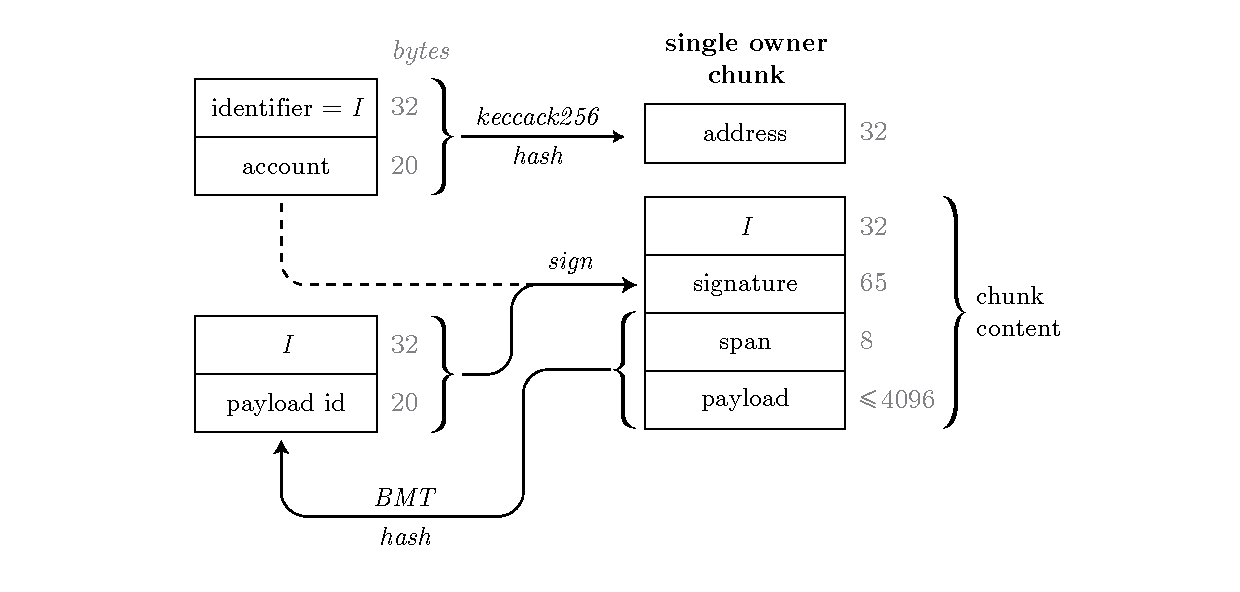
\includegraphics[width=\textwidth]{single-owner-chunk.pdf}
  \caption{Single owner chunk (SOC). Unlike content-addressed chunks, SOCs obtain their integrity through the signature of their (single) owner and cross-owner immutability through hashing the owner's address in the chunk address (effectively achieving access control via namespacing).}
   \label{fig:soc}
  \end{figure}

The address of a SOC is by its definition the hash of, its ID and the Ethereum address of its owner. In order to create valid SOCs, uploaders need to sign the SOC with the owner's identity. Therefore in our case, for replication, the owner of the SOC must be a consensual identity with their private key publicly revealed, for the system to be able to create SOC-based replicas.
%
\footnote{This has the added benefit that third parties can also upload replicas of any chunk.}

The first component of the address, the SOC ID, must, to be useful for replication, satisfy two new criteria: (1) it needs to match the payload hash up to 31 bytes and (2) it must provide the entropy needed to mine the overall chunk into a sufficient number of distinct neighbourhoods. (1) is added as a validation criterion for the special case of replica SOCs, while (2) takes care that replicas are stored uniformly dispersed within the address space.
This construct is called \emph{dispersed replica}:

Let us assume $c$ is the content-addressed chunk we need to replicate; $n$ is the number of bits of entropy available to find the nonces that generate  $2^k$  perfectly balanced replica. We initialize a chunk array $\rho$ of length $2^k$, the elements of which we will call \emph{bins} and start with $n$-bit integer nonce $i=0$ and replica counter $C=0$.

\begin{enumerate}[noitemsep]
  \item Create the SOC ID $id$ by taking $\textsc{Address}(c)$ and change the last byte (at index position 31) to  $i$.
  \item Calculate the SOC address $a_i$ by concatenating SOC ID $id$ and the SOC owner constant $o$%
%
\footnote{The SOC owner of dispersed replicas has the arbitrary private key $\texttt{0x010...00}$
and the corresponding ether address is
$o = 0xdc5b20847f43d67928f49cd4f85d696b5a7617b5$.}
%
and hashing the result using the Keccak256 base hash $a_i=H(id\concat o)$, and record $c_i=\mathit{SOC}(id,o,c)$.
  \item Calculate the bin that $a_i$ belongs to by taking the $k$-bit prefix as big-endian binary number $j<2^k$.
  \item If $\rho\idx{j}$ is unassigned, then let $\rho\idx{j}:=c_i$ and increment $C$.
  \item If $C=2^k$, then quit.
  \item Increment $i$ by one, if $i=2^n$, then quit.
  \item Repeat from Step 1.
\end{enumerate}

With this solution, we are able to provide an arbitrary level of redundancy for the storage also of data smaller or equal to a chunk's size (4K). As the previous schema scales indefinitely, we now have a combined mechanism for all data sizes.
%
%
\footnote{Note that if $n$ is small, then generating all $2^k$ balanced replicas may not be achievable, and if $n<k$, this is certainly not possible.
In general, given $n, k$ at least $m$ miss has a probability of $(1 - m/2^k)^{2^n}$.}

Depending on the strategy, the downloader can choose which  address to retrieve the chunk from. The obvious choice is the replica closest to the requesting node's overlay address $a_r$. In other words, the last item of the sorted chunk array $\rho$ using the comparison function:
\begin{equation}
  i<j\Leftrightarrow    	
  \mathit{PO}(a_r,
  \textsc{Address}(\rho\idx{i}))
  <\mathit{PO}(a_r,
  \textsc{Address}(\rho\idx{j}))
\end{equation}


% \section{The special case of a single chunk} \label{sec:the-special-case-of-a-single-chunk}

If the probability of any replica being faulty is $\epsilon$, then, assuming independence, the probability that $n$ parities are faulty is $\epsilon^n$. Here we can write $n = k + 1$; that is, we have one ``original'' chunk and the rest of them are the $k$ parities. Keeping the overall error probability below $\alpha$ then means that
\begin{equation}
%%%%%%%%%%%%%%%%%%%%
  \epsilon^{k+1} = \alpha
  \label{eq-onechunk}
\end{equation}
must be satisfied. Taking logarithms on both sides and rearranging, we get
\begin{equation}
  k = \frac{\log(\alpha)}{\log(\epsilon)} - 1 .
  \label{eq-onechunk-parities}
\end{equation}
This is the number of parities of a singleton chunk required to keep the overall data corruption probability below $\alpha$. The base of the log in Equation~\ref{eq-onechunk-parities} is arbitrary. This means that if we use base-10 logarithms and assume that $\alpha = 10^{-6}$, for $\epsilon < 1$ (error rate < 100\%), we get the simpler
\begin{equation}
  k  = \frac{-6}{\log_{10}(\epsilon)} - 1 = \frac{6}{|\log_{10}(\epsilon)|} - 1 .
  \label{eq-onechunk-special}
\end{equation}
For example, if the per-chunk error rate is ten percent ($\epsilon = 0.1$), then $|\log_{10}(\epsilon)| = |\log_{10}(1/10)| = 1$, and so $k = 6/1 - 1 = 5$ parities are needed. If instead the per-chunk error rate is just one percent ($\epsilon = 0.01$), then only $k = 6/2 - 1 = 2$ parities are necessary.

In particular, for the same per-chunk error rates as in Table~\ref{tbl:levels}, we get:
\begin{table}[!ht]
\caption{For a given per-chunk error rate (first column), how many parities (second column) are required of a single chunk to keep the overall data corruption probability below $\alpha = 10^{-6}$?}
\begin{center}
\begin{tabular}{|l|r|r|r|}
\hline
\multicolumn{1}{|c|}{\multirow{2}{1.5cm}{\centering security\\level}} &
\multicolumn{1}{|c|}{\multirow{2}{1.5cm}{\centering error\\rate}} &
\multicolumn{1}{|c|}{\multirow{2}{1.5cm}{\centering parities\\required}} &
\multicolumn{1}{|c|}{\multirow{2}{1.6cm}{\centering dispersed\\replicas}}\\&&&\\\hline\hline
\textsc{none} & 0\%     & 0 & 0  \\
\textsc{medium} &   1\% & 2 & 2\\
\textsc{strong} &   5\% & 4 & 4 \\
\textsc{insane} &   10\% & 5 & 8 \\
\textsc{paranoid} & 50\% & 19 & 16\\
\hline
\end{tabular}
\end{center}
\label{tbl:single-chunk}
\end{table}



\section{Prefetching strategies for retrieval}
\label{sec:strategies}

When downloading, systematic per-level erasure codes allow for performance-optimizing \emph{prefetching strategies}:
\begin{labelledlist}
\item[\textsc{NONE} = \emph{direct with no recovery; frugal}] No prefetching takes place, RS parity chunks are ignored if present. Retrieval involves  only the original chunks, no recovery. 
\item[\textsc{DATA} = \emph{prefetching data but no recovery; cheap}] Prefetching only original chunks, RS parity chunks are ignored if present, no recovery.
\item[\textsc{PROX} = \emph{distance-based selection; cheap}] For all intermediate chunks, first retrieve $ m$ chunks that are expected to be the fastest to download (e.g. the $m$ closest to the node). This optimizes performance by potentially reducing overall hops required and the number of nodes involved, at the cost of calculating distances and resolving RS codes to reconstruct the data from the arbitrary set of $m$ chunks that happened to be closest.
\item[\textsc{RACE} = \emph{latency optimized; expensive}] Initiate requests for all chunks within the scope (max $m+k$). Wait only for the first $m$ chunks delivered in order to proceed. This is equivalent to saying that the $k$ slowest chunk retrievals can be ignored. This strategy is optimal for latency, in case some chunks arrive faster even though they are not among the closest $m$. Like for $PROX$, RS codes are resolved. Both processing and bandwidth are maximized to achieve fastest possible delivery.
\end{labelledlist}

% ALTERNATE
%
% Either 2 levels should be added or retrieval fallback be kept out of this as separate setting.
% Because, whether prefetching uses replica or not, when something went wrong, fetching could still fallback to using replicas. This is lumped into one in NONE and DATA.
%
% There could even be 2 more levels, because PROX and RACE could also decide to fix errors using replica (that will arrive later, thus lose speed at that moment) or ignore that (e.g. for videos).
%
% Yet another level mode could have error correction happening already during prefetching, as soon as an error is detected (from the content-address).
%
% Ether way, the decision to error correct or not is logically separate from prefetching strategy. 'Retrieval involves  only the original chunks, no recovery.' does not belong here.
%
%
% The following assumes a separate switch to decided about error correction after prefetching and thus deletes such sentences:

% When downloading, systematic per-level erasure codes allow for performance-optimizing \emph{prefetching strategies}:
%
% Note that the decision to error correct or not, using the replica, after the prefetching is potentially governed by a separate setting and not determinted by the settings listed below.
%
% \begin{labelledlist}
% \item[\textsc{NONE} = \emph{direct with no recovery; frugal}] No prefetching takes place. 
% \item[\textsc{DATA} = \emph{prefetching data but no recovery; cheap}] Prefetching only original chunks, RS parity chunks are ignored during prefetching. No recovery (yet) during prefetching.
% \item[\textsc{CORR} = \emph{prefetching data with recovery; cheap}] Prefetching original chunks, falling back to RS parity chunks if errors are detected (i.e. simply, when address and content hash don't match).
% \item[\textsc{PROX} = \emph{distance-based selection; cheap}] For all intermediate chunks, first retrieve $m$ chunks that are expected to be the fastest to download (e.g. the $m$ closest to the node). This can optimize performance by potentially reducing overall hops required and the number of nodes involved, at the cost of calculating distances and resolving RS codes to reconstruct the data from the arbitrary set of $m$ chunks that happened to be closest. Error correct using the remaining chunks as needed.
% \item[\textsc{RACE} = \emph{latency optimized; expensive}] Initiate requests for all chunks within the scope (max $m+k$). Wait only for the first $m$ chunks delivered in order to proceed. This is equivalent to saying that the $k$ slowest chunk retrievals can be ignored. This strategy is optimal for latency, in case some chunks arrive faster even though they are not among the closest $m$. Like for $PROX$, RS codes are resolved. Both processing and bandwidth are maximized to achieve fastest possible delivery. Error correcting happens as needed using the remaining chunks.
% \end{labelledlist}


Note that while they are based on a resilience mechanism, $PROX$ and $RACE$ are excellent performance architectures, which has been shown in practice through live video streams on Swarm. Dropped packages are easily overcome without visible quality dip in these prefetch modes.

All in all, strategies using recovery can effectively overcome the occasional unavailability of chunks, be it due to faults such as network contention, connectivity gaps in the Kademlia table, node churn, overpriced neighborhoods, or even malicious attacks targeting a specific neighborhood. 

Similarly, given a typical model of network latencies for chunk retrieval, erasure codes in \textsc{RACE} mode can guarantee that minimal possible retrieval latencies are achieved.%
%
\footnote{For instance, in the temporally sensitive case of real-time video streaming, for any quality setting (bitrate and FPS), buffering times can be guaranteed if the batch of chunks representing a time unit of media is encoded using its own scope(s) of erasure coding.}


\section{Conclusion}\label{sec:conclusion}

This work presents a comprehensive strategy for enhancing data availability in decentralized storage by embedding erasure coding directly into the Swarm chunk tree. By enabling Reed–Solomon encoding at the level of packed address chunks, the system achieves non-local redundancy without compromising the deterministic structure of content addressing. The construction allows for user-configurable security levels, defined by quantifiable probabilities of successful retrieval, and supports efficient decoding even under partial network failure. For edge cases involving singleton chunks, the introduction of dispersed replicas ensures resilience through address-space diversification. Furthermore, a spectrum of retrieval strategies is proposed that can exploit the replication mechanism to balance cost, latency, and robustness depending on application needs. Together, these mechanisms form a robust foundation for scalable, fault-tolerant and high-performance storage in unreliable or adversarial environments.

%%
%% The acknowledgments section is defined using the "acks" environment
%% (and NOT an unnumbered section). This ensures the proper
%% identification of the section in the article metadata, and the
%% consistent spelling of the heading.
\begin{acks}
We thank Andrea Robert for her comments and thorough editing work which have greatly improved the paper.
\end{acks}

%%
%% The next two lines define the bibliography style to be used, and
%% the bibliography file.
\bibliographystyle{ACM-Reference-Format}
\bibliography{refs}


%%
%% If your work has an appendix, this is the place to put it.
% \appendix

% \section{Research Methods}

% \subsection{Part One}

% Lorem ipsum dolor sit amet, consectetur adipiscing elit. Morbi
% malesuada, quam in pulvinar varius, metus nunc fermentum urna, id
% sollicitudin purus odio sit amet enim. Aliquam ullamcorper eu ipsum
% vel mollis. Curabitur quis dictum nisl. Phasellus vel semper risus, et
% lacinia dolor. Integer ultricies commodo sem nec semper.

% \subsection{Part Two}

% Etiam commodo feugiat nisl pulvinar pellentesque. Etiam auctor sodales
% ligula, non varius nibh pulvinar semper. Suspendisse nec lectus non
% ipsum convallis congue hendrerit vitae sapien. Donec at laoreet
% eros. Vivamus non purus placerat, scelerisque diam eu, cursus
% ante. Etiam aliquam tortor auctor efficitur mattis.

% \section{Online Resources}

% Nam id fermentum dui. Suspendisse sagittis tortor a nulla mollis, in
% pulvinar ex pretium. Sed interdum orci quis metus euismod, et sagittis
% enim maximus. Vestibulum gravida massa ut felis suscipit
% congue. Quisque mattis elit a risus ultrices commodo venenatis eget
% dui. Etiam sagittis eleifend elementum.

% Nam interdum magna at lectus dignissim, ac dignissim lorem
% rhoncus. Maecenas eu arcu ac neque placerat aliquam. Nunc pulvinar
% massa et mattis lacinia.

\end{document}


\endinput
%%
%% End of file `sample-manuscript.tex'.
